\section{Environmental model}

In order to estimate the behavior of an object in natural environment, the ambient effects must be estimated first. The two major environmental factors are the effects of the sea and wind. They generate periodic loads that stirs and slowly wears down objects they come in contact width. An ocean surface is almost never still, as waves carry the memory of distant and past storms for a long way. However, the ever-changing and chaotic surface of the sea is composed of regular waves, each having its own frequency, direction and amplitude.

\subsection{Wave model} A simple, but adequately complex irregular wave model\cite[p.~14]{shipsim} can be derived from the basic hydrodynamic principles using superposition of regular waves\cite[p.~19]{hydromechanics}.

\begin{align}
		\zeta (x, y, t) = T + H_s * \sum_{i=1}^{10} (cos(k .* (x .* sin(\chi) + y * cos(\chi)) + \Omega * \omega{_i} * t + \Phi))
\end{align}

By computing the current water height at every surface points, it's possible to visualize the qeuation above:

\begin{figure}[H]
	\centering
	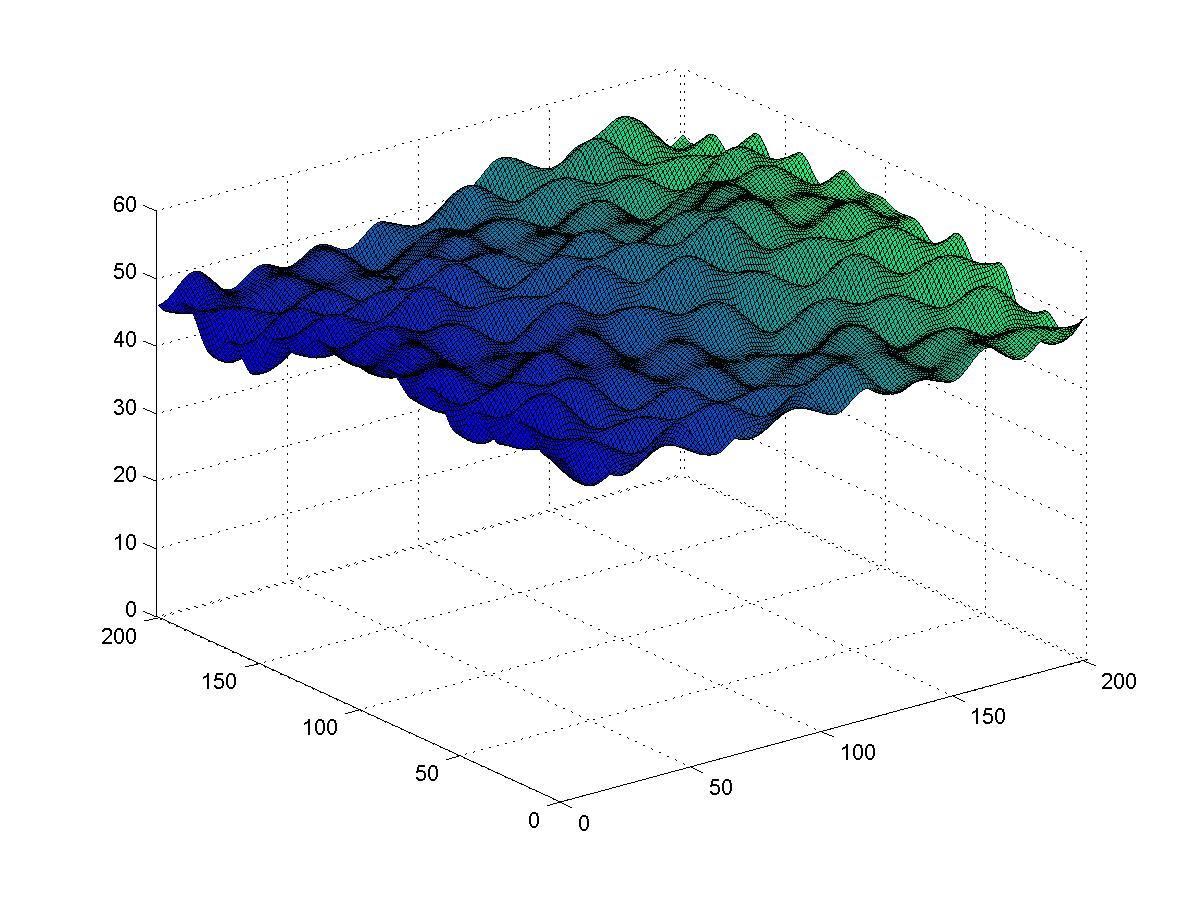
\includegraphics[width=0.8\textwidth]{fig/wavemodel}
	\caption{Simulation result of the irregular wave model}
	\label{fig:wavemodel}
\end{figure}

\subsection{Wind model}

TODO: Beaufort-scale, wind-waves

\subsection{Behaviour of objects in waves}

The movement of ships in water is the result of a number of external forces, like gravity, buoyancy, waves, wind, etc. and the damping effect of the inertia of the ship.

Behaviour in water can be separated to six different motions.

3 translational:

\begin{itemize}

	\item \emph{Surge} in the longitudinal \textbf{x}-direction, positive forwards
	\item \emph{Sway} in lateral \textbf{y}-direction, positive to port (left) side
	\item \emph{Heave} in the vertival \textbf{z}-direction, positive upwards

\end{itemize}

and 3 rotational:

\begin{itemize}

	\item $\Phi$ - \emph{Roll} around the longitudinal \textbf{x}-axis, positive right turning
	\item $\Theta$ - \emph{Pitch} around lateral \textbf{y}-axis, positive right turning
	\item $\Psi$ - \emph{Yaw} around the vertival \textbf{z}-axis, positive right turning

\end{itemize}

These components are built up of multiple sub-components possessing small amplitudes and different frequencies.

[img from ShipHydromechanics 38.pg perhaps?]

In hydrodynamics, the geometrical extent of the floating body must be considered. A wave traveling beneath the ship acts as a force distributed in space and time, first pushing the bow, then the stern of the ship upwards. By sarcificing precision, the approximate forces acting on the hull can be modeled using several approximation points.

Let's introduce the dynamic model of a floating rigid body. As stated earlier, it has 6 movements, which results in 6 state variables:

[table: x1:Surge, x2: Sway, x3: Heave, x4:Roll, x5:Pitch, x6:Yaw]

For each state variable, a state-transition equation can be defined based on external forces:

\begin{align}
	\dot{Surge}_{x_1} &= \frac{F_F}{m} \\
	\dot{Sway}_{x_2}  &= \frac{F_S}{m} \\
	\dot{Heave}_{x_3} &= \frac{F_V}{m} \\
	\dot{Roll}_{x_4}  &= \frac{T_x}{I_x} \\
	\dot{Pitch}_{x_5} &= \frac{T_y}{I_y} \\
	\dot{Yaw}_{x_6}   &= \frac{T_z}{I_z}
\end{align}

Now the problem is simplified to determining the external forces affecting the body. In order to do this, we apply Archimedes' law\cite{archimedes} on a number of control points. Let's start with 4 points, distributed equally from each other and the edges of a rectangular body.

[illustration (Autodesk Inventor?)]

Each control point has a position and height that can be determined based on the state variables and it's position on the surface of the object, using trigonometrical functions. Moreover, each control point has a constant volume, that depends on the volume of the initial object and the number \& distribution of control points. In order to compute the actual positions of the control points, we use the 3D rotation formula.

\begin{align}
	R_x(\Theta) = 
	\begin{bmatrix}
		1 & 0 & 0 \\
		0 & \cos \Theta & -\sin \Theta \\
		0 & \sin \Theta & \cos \Theta
	\end{bmatrix} \\
	R_y(\Theta) = 
	\begin{bmatrix}
		\cos \Theta & 0 & \sin \Theta \\
		0 & 1 & 0 \\
		\sin \Theta & 0 &\cos \Theta
	\end{bmatrix}
 \\
	R_z(\Theta) = 
	\begin{bmatrix}
		\cos \Theta & \sin \Theta & 0 \\
		\sin \Theta & \cos \Theta & 0 \\
		0 & 0 & 1
	\end{bmatrix}
\end{align}

It's possible to combine the three rotation matrices into a single formula, but I believe it's more structured and easier to work width when kept separate. Using these formulae the position of a single control point, relative to the ship's centre of mass:

\begin{align}
	\begin{bmatrix}
		C_x \\
		C_y \\
		C_z
	\end{bmatrix}
	 = R_x(\Phi) * R_y(\Theta) * R_z(\Psi) *
	\begin{bmatrix}
		C_a \\
		C_b \\
		C_c
	\end{bmatrix}
\end{align}

Where a, b and c represents the coordinates in the \textbf{body} frame, while x, y and z represents the coordinates in the \textbf{local} coordinate system. Now that the \textbf{relative} positions of the control points are known, to obtain the \textbf{world} coordinates of the points, they must be offset with the position of the body.

\begin{align}
	\begin{bmatrix}
		W_x \\
		W_y \\
		W_z
	\end{bmatrix}
	=
	\begin{bmatrix}
		C_x \\
		C_y \\
		C_z
	\end{bmatrix}
	 =
	\begin{bmatrix}
		S_x \\
		S_y \\
		S_z
	\end{bmatrix}\\
	\textbf{W} = \textbf{C} + \textbf{S}
\end{align}

Now we only have to solve the wave model equation in these points only, to determine the current approximated waterline. Based on the sinkage of each control point, the current force of buoyancy can be approximated. This force is not always vertical, but normal to the surface of the wave, thus generating not only torque, but slight translational movement as well. It's important to note, that the buoyant forces are calculated based on volume, but the torques are affected by these forces and the center of gravity as well.

\paragraph{Damping} As it should have become trivial by now, the motion of the ship, just like the the sea, is the superposition of a number of harmonic movements. The friction, torrents and other effects dampen this oscillation. In order to approximate these restricting forces, the model must be extended with other elements.

\section{Maneuvering model}

Simple ship dynamic models can be formulated quickly by defining and analyzing the most common propulsion methods. However, these are only vague approximations of the system, and contain few elements of the complex and powerful hydrodynamics.

First the simple ship models are introduced, then an attempt is made to more accurately describe the dynamical system of a ship.

\subsection{Differential drive}

The differential drive system is very common among simple mobile robotic systems. The movement is based on two separately driven wheels placed on either side of the robot body. It can thus change its direction by varying the relative rate of rotation of its wheels, therefore does not require an additional steering mechanism. A twin-screw ship has a somewhat similar layout. Using the engines positioned in a lateral offset to the centerline of the body, the ship can create a torque and propelling force affecting the body.

[figure about diff drive]

This type of ship can be modeled as a 2-DOF mobile robot (frame fixed to the body of the ship).

The dynamical system of the parallel propulsion engines can be formulated easily:

Figure here! d is the distance of the wheel from the center

\begin{align}
	\dot{x} &= \frac{v_1}{2} + \frac{v_2}{2} \\
    \dot{\Theta} &= \frac{v_1-v_2}{2*d}
\end{align}

From a control engineer’s point of view the most important aspect of this control system is its linearity. Designing a basic controller for this type of robot is a walk in the park.

The mechanical advantage of this layout is the very high reliability, because the propellers are fixed in a certain angle, therefore they can be build more roboustly, thus decreasing the chance of physical failture. Another advantage is the ability of the ship to turn around it’s central axis, enabling precise maneuvering, however, this is seldom used, because it’s very ineffective with ships.
Usually older large container-ships employ this type of propulsion. Newer large-scale ship design have kept the multi-screw layout, but also included a rudder directly after the propellers to enhance turning.

\subsection{Rudder}

The rudder is a controllable part of the ship, creating a tourque on the body of the ship, using hydrodynamical effects, much like the rudders of airplanes. The generated torque depends on the traveling speed. A ship like this can usually not rotate around it’s center axis, nor travel backwards efficiently.

A representation of a rudder ship can be modeled as a surface car with Ackermann steering. This model is very vague, but is useful for the testing of the higl level course controller and pathplanning.

\begin{align}
	\dot{x} &= v \\
	\dot{\Theta} &= \frac{v * tan(\Phi)}{L}
\end{align}

The type of the rudder and its placement have a major effect on the controllability of the ship.

[rudder types figures]

All sorts of rudders are required to produce large turning forces, but the rudder size must be balanced between to a good generated torque to draft ratio.
To determine the approximate size of an optimal rudder for a given ship, a certain rule of thump value of Det Norske Veritas for a minimum projected rudder area can be applied:

\begin{align}
	A_r approx&= \frac{d * Lpp}{100}(1.0 + 25.0 * (frac{B}{L_{pp}})^2)
\end{align}

where:

\begin{align}
	A_r &= projected rudder area \\
	L_{pp} &= length between perpendiculars \\
	B &= beam \\
	d &= draft
\end{align}

"This formula 4.1 applies only to rudder arrangements in which the rudder is located directly
behind the propeller. For any other rudder arrangement Det Norske Veritas requires an
increase in the rudder area by - at least - 30 percent. A twin screw (or more) arrangement
should be combined with rudders located directly behind the propellers for maximum lowspeed
maneuverability. A single rudder placed between two propellers may be inadequate,
because the rudder blade does not swing su¢ciently into the ‡ow of a propeller to generate
the needed turning moment." (copied, to restructure)

The rudder of the ship acts as an airfoil that produces lift and drag. The [figure] shows a rudder placed in constant flow. The total force can be decomposed. (nem értem, 55. oldal ship hydromechanics)

\begin{align}
	C_L &= projected rudder area \\
	L_{pp} &= length between perpendiculars \\
	B &= beam \\
	d &= draft
\end{align}

[figure: rudder forces]

\subsection{Sailing ship}

The sailing ship is usually controlled by the rudder. It’s possible to alter the course by adjusting the sails or tilting the mast (e.g.: windsurfing). the center of the sails is shifting, and will produce a torque around the center of lateral surface.
There are many forces affecting the sails and the body of the ship, but it’s way out of the scope of this text to model all of them. However, they can be generalized in two forces, the lift and the drag.

Lift is the force generated on the sails by the wind, affecting paralell with the body of the ship, and drag is the force generated perpendicular to the body of the ship. These forces are greatly and nonlinearly dependent on the strength and direction of the wind, current speed, air pressure, wind shears, body drift and keel form, local temperature gradients and other circumstances.

Simulating all these effects is a scientific field of its own. Instead, we are using polar sailing diagrams to approximate the maneuvering performance of the boat. These diagrams, often used as a marketing tool are a widespread visual representation of the capabilities of a specific ship. By allowing the software to process these diagrams, the controller and pathplanner can be effectively customized.

The resulting software is heavily based on the supplied sailing diagram, but automatic calibration is also possible using wind sensors and GPS.

\begin{align}
		\dot{x} &= v_x
	\\	\dot{y} &= v_y
	\\	\dot{v}_x &= lift - \frac{v_x}{bodydrag_x}
	\\	\dot{v}_y &= drag - \frac{v_y}{bodydrag_y}
	\\	\dot{\Theta} &= \frac{v_x * tan(\Phi)}{L}
\end{align}

\subsection{Building simulation environment}

Based on a survey completed in the Brazilian and United States Navy the importance of various aspects of the simulation can be determined\cite[p.~6]{shipsim}. The result of the analysis show that the most essential areas are the acceleration, deceleration and turning rates of the ship. According to the respondents the simulation of the possible visibility issues are also important, and the environmental effects also scored high on the priority list. The results indicate that that the distribution and the wake of ship is less significant in a virtual environment.

\begin{tcolorbox}[colback=cyan!5,colframe=cyan!40!black,title=Code: Simulator.py \\ https://www.dropbox.com/s/agron9anslev6xw/Simulator.py]
\begin{minipage}{0,6\textwidth}
According to the guidelines of the seamless simulator, this part of the system has its own distinctive object. Everything related to the simulator and everything that is unknown during the mission is stored and handled here.
\end{minipage}
\begin{minipage}{0,35\textwidth}
\raggedleft

\includegraphics[width=0.8\textwidth]{img/simulatorcode}
\end{minipage}
\end{tcolorbox}

\subsection{Uncontrolled system simulation results}